\documentclass[journal]{IEEEtran}

\usepackage{cite}
\usepackage[utf8]{inputenc}
\usepackage[T1]{fontenc}
\usepackage{url}
\usepackage{booktabs}
\usepackage{amsfonts}
\usepackage{nicefrac}
\usepackage{microtype}
\usepackage{xcolor}
\usepackage{graphicx}
\usepackage{tabularx}
\usepackage{array}
\usepackage{hyperref}

\graphicspath{{figures/}}

\newcommand{\metric}[1]{\texttt{#1}}

\title{Runtime-Constrained Evaluation of Fine-Tuned Local LLM Driving Agents for Intelligent Vehicles}

\author{Anjie~Qiu%
\thanks{Anjie Qiu is with the Department of Electrical and Information Technology, RPTU Kaiserslautern-Landau, 67663 Kaiserslautern, Germany (e-mail: qiu@eit.uni-kl.de).}}

\markboth{IEEE Transactions on Intelligent Vehicles, under review}%
{Qiu: Runtime-Constrained Evaluation of Fine-Tuned Local LLM Driving Agents}

\begin{document}

\maketitle

\begin{abstract}
Evaluation of large language model driving agents for intelligent vehicles is constrained not only by task quality, but also by whether local runtime behavior leaves runs comparable in the first place. This paper presents DiLu-Ollama as a local-first evaluation framework for studying fine-tuned LLM driving agents under a shared highway benchmark while treating benchmark validity as part of the measured outcome. The framework combines local inference, task-conditioned highway simulation, and a post-hoc analysis pipeline that records task metrics together with ranking eligibility, invalidity reasons, and latency behavior. Using this framework, we study lightweight, midclass, and highclass model tiers under one runtime regime and find a sharp interpretability boundary: lightweight is the only tier that supports stable comparative ranking, midclass remains screening-only, and all tested 14B models fail ranking eligibility under the current local setup. Within the valid region, the lightweight Phi pair provides the only exact base-versus-fine-tuned comparison and shows that fine-tuning can improve driving score without an obvious mean-latency penalty. These results position benchmark validity as a first-class requirement for automated-vehicle evaluation of local LLM agents and show that fine-tuning claims are only trustworthy where the evaluation regime itself remains stable.

\end{abstract}

\begin{IEEEkeywords}
Intelligent vehicles, autonomous driving, large language models, local inference, benchmark validity.
\end{IEEEkeywords}

\section{Introduction}

Evaluation for intelligent vehicles has long relied on simulation and scenario-based testing because exhaustive real-world validation is infeasible, expensive, and slow to reproduce \cite{riedmaier2020scenario}. That challenge becomes sharper when the decision-making component is a large language model. Recent work has shown that LLMs can serve as planners, controllers, or interpretable decision interfaces in autonomous-driving settings \cite{wen2023dilu,sha2023languagempc,fu2023drivelikehuman,xu2023drivegpt4}. However, once these agents are evaluated under local deployment constraints, task quality is no longer the whole story. Fixed inference budgets, timeout escalation, and fallback behavior can change whether a run remains comparable at all.

This issue matters directly for automated-vehicle evaluation practice. In simulation studies, benchmark rankings are often used to choose controller variants, adaptation strategies, or the next round of validation effort. If invalid runs are silently filtered or interpreted as ordinary score outliers, the evaluation can recommend models that do not remain operational under the runtime regime in which they are actually deployed. Prior work on consumer-grade LLM serving already shows that practical usability depends heavily on hardware-aware runtime behavior \cite{song2023powerinfer}. In local intelligent-vehicle evaluation, that same runtime behavior determines which empirical conclusions survive scrutiny.

Fine-tuning makes this measurement problem more important rather than less. Parameter-efficient methods such as QLoRA make local adaptation feasible on limited hardware \cite{dettmers2023qlora}. But an adapted model is only meaningfully better if its gain survives the runtime regime used to measure it. Broader model evaluation work has already argued that trustworthy assessment requires more than a single aggregate score \cite{liang2022helm}. In our setting, that principle takes a concrete form: if fine-tuning improves action quality but pushes a local driving agent into timeout collapse, the correct conclusion is not a simple fine-tuning win, but a tradeoff between policy quality and benchmark validity.

DiLu-Ollama addresses this problem by combining a DiLu-style driving decision loop with local Ollama inference, \metric{highway-env} simulation, a task-conditioned highway benchmark, and a post-hoc study pipeline that preserves invalidity and failure context rather than hiding it \cite{wen2023dilu,leurent2018highwayenv}. We use that pipeline to study whether fine-tuning improves small-to-mid local driving models under a shared three-tier highway benchmark. The evidence is deliberately narrow: highway only, no cross-scenario empirical claims, and pairwise fine-tuning conclusions restricted to exact ranking-eligible base-versus-tuned pairs. Under those rules, the usable evidence is concentrated in lightweight, where the Phi family yields one exact eligible improvement. Midclass remains screening-only, and highclass becomes a meaningful result of its own: the point where the benchmark regime is fragile enough that competitive ranking claims are no longer justified.

This paper makes three contributions. First, it presents a local-first evaluation and analysis scaffold for intelligent-vehicle LLM agents in which benchmark validity is part of the empirical outcome. Second, it provides a three-tier study showing that benchmark viability degrades with model tier under a fixed local runtime policy. Third, it provides initial but concrete evidence that fine-tuning can improve local driving agents in lightweight settings while making explicit where broader family-level claims are still blocked.

\section{Related Work}

Automated-vehicle evaluation literature has emphasized for years that scenario-based simulation is not just a convenience layer, but a core methodological instrument for establishing trustworthy performance and safety claims \cite{riedmaier2020scenario}. That literature typically focuses on coverage, scenario selection, and validation logic at the vehicle-system level. Our work is aligned with that concern, but addresses a newer source of evaluation fragility: the runtime instability introduced when the driving policy itself is a locally deployed large language model.

Recent work has established that large language models can act as high-level decision components for autonomous driving, but the literature is still split between papers that emphasize behavioral capability and papers that emphasize interpretability or system design. Early work such as \emph{Drive Like a Human} argued that language models can serve as driving-policy interfaces rather than pure text processors \cite{fu2023drivelikehuman}. Follow-up systems including DiLu, LanguageMPC, and DriveGPT4 broadened that direction by treating language models as planners, decision makers, or interpretable end-to-end controllers in simulated driving settings \cite{wen2023dilu,sha2023languagempc,xu2023drivegpt4}. A recent survey, \emph{LLM4Drive}, makes clear that this area is expanding quickly across planning, perception-language interaction, and embodied control \cite{yang2023llm4drive}. Our paper is closest to this line of work, but differs in emphasis: we do not primarily ask whether an LLM driving agent can complete a scenario. We ask when the local evaluation regime remains valid enough for those comparisons to be trusted.

That distinction also changes how we use the fine-tuning literature. Parameter-efficient adaptation methods such as LoRA and QLoRA make it feasible to specialize local language models without full retraining \cite{hu2021lora,dettmers2023qlora}. Systems work on local inference, including PowerInfer, further shows that practical deployment quality depends heavily on hardware-aware runtime behavior rather than model capability in isolation \cite{song2023powerinfer}. Broader evaluation work such as HELM argues that meaningful model comparison requires multiple dimensions of assessment rather than single-score reporting \cite{liang2022helm}. DiLu-Ollama sits at the intersection of these threads. It studies fine-tuned local driving agents, but evaluates them through a benchmark that preserves invalid runs, timeout collapse, and latency-induced comparability failures.

\section{Benchmark and Framework Setup}

DiLu-Ollama extends the DiLu driving-agent loop into a local-first evaluation stack built on Ollama inference, \metric{highway-env}, and a benchmark-oriented reporting pipeline \cite{wen2023dilu,leurent2018highwayenv}. For this paper, we use only the highway benchmark path. Each run produces task metrics such as \metric{driving\_score\_v2}, task completion, and crash rate, together with latency and ranking-eligibility metadata. We treat that eligibility signal as part of the measurement outcome, because invalid runs in the current setup are often direct consequences of timeout escalation and latency collapse rather than random noise. Figure~\ref{fig:local-eval-validity-pipeline} summarizes this measurement path and makes the validity gate explicit: invalid runs are retained for screening and failure analysis rather than being silently removed before interpretation. Table~\ref{tab:validity-summary} therefore summarizes not only performance but also whether comparison remains methodologically sound across tiers.

\begin{figure}[t]
\centering
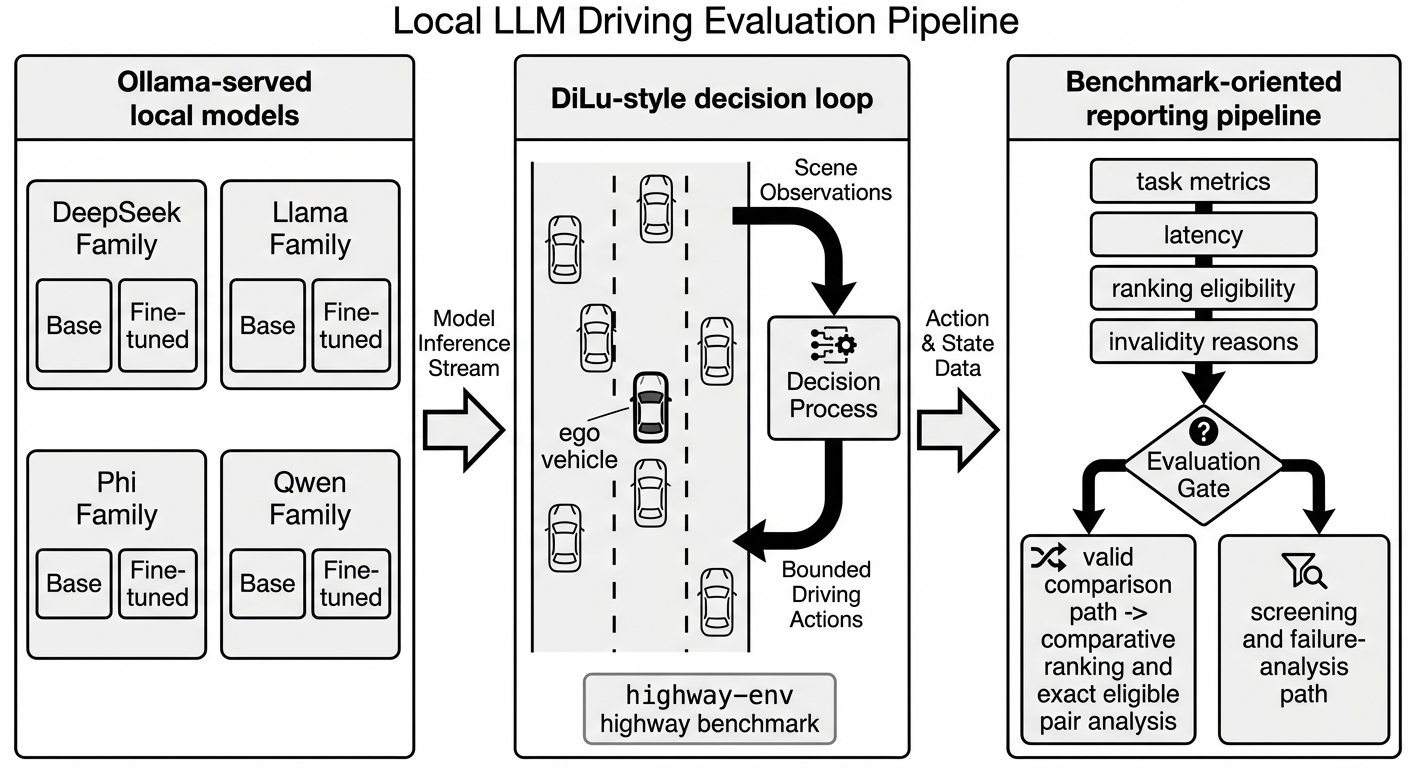
\includegraphics[width=\linewidth]{local_eval_validity_pipeline.png}
\caption{Local evaluation and validity-handling pipeline. The figure shows the highway-only measurement path from Ollama-served local model families through the DiLu-style decision loop in \metric{highway-env} to benchmark-oriented reporting. Crucially, invalid runs are retained as outcomes and routed to screening or failure analysis rather than being silently filtered out.}
\label{fig:local-eval-validity-pipeline}
\end{figure}

This distinction matters for intelligent-vehicle evaluation. A simulation benchmark is often expected to function as a comparative instrument for controller or policy selection. In the local LLM setting, however, the benchmark must also reveal when runtime behavior prevents that comparison from being fair or reproducible. DiLu-Ollama is designed to expose that failure boundary explicitly rather than hide it behind post-processing.

The repository now also contains discrete cross-scenario support for merge and intersection environments, but those results are outside the evidential scope of this paper. All empirical claims below are tied to the current three-tier highway study bundle.

With that benchmark boundary fixed, the next question is which fine-tuning comparisons remain valid enough to interpret.

\section{Fine-Tuning Setup}

The repository fine-tuning path is intentionally local-first. Training begins with expert highway trajectories collected under the same task family used for evaluation, then converts those trajectories into a strict instruction-output format suitable for supervised adaptation. The pipeline subsequently rebalances the action distribution, validates row schema and action formatting, produces merged model exports after training, and packages those exports for local deployment through GGUF conversion and Ollama model creation. This sequence matters for the paper because the evaluated fine-tuned models are not abstract checkpoints: they are deployment-oriented local artifacts produced by the same toolchain that a practitioner would use to run the benchmark end to end.

The training implementation is compatible with efficient adaptation in the QLoRA line \cite{dettmers2023qlora}, but the paper does not claim novelty in the optimizer or adapter mechanism itself. The methodological question is instead whether locally adapted models remain meaningfully comparable once they are placed back under the same runtime-constrained driving benchmark. For that reason, the fine-tuning section is primarily about comparison control rather than optimization design.

To make that comparison explicit, the study organizes models through a registry that records family, tier, \texttt{variant\_kind}, and a \texttt{base\_model\_id} link from each fine-tuned artifact back to its intended base model. This registry provides nominal lineage and lets the post-hoc study pipeline recover base-versus-fine-tuned pair structure after benchmark execution. Lineage alone, however, is not enough for scientific comparison. We make pairwise fine-tuning claims only when both sides of a family remain ranking-eligible under the same benchmark regime. This rule is a methodological control, not merely a reporting preference: if either the base model or the adapted model falls out of the valid ranking set, then a base-versus-tuned delta can be driven by timeout collapse or invalid execution rather than adaptation quality.

Under the current publication bundle, the only exact eligible pair is the lightweight Phi family. The paper should therefore be read as an initial fine-tuning study with narrow but real causal evidence, not as a complete family-by-family adaptation benchmark. Lightweight scale still supports one direct before-and-after comparison under shared runtime conditions. Midclass and highclass, by contrast, still contain training artifacts and registry-defined lineages, but they do not preserve the benchmark conditions needed for equally strong pairwise interpretation. That boundary is central to the paper's methodology: we compare only where the benchmark still behaves like a benchmark, and we treat the loss of pairwise comparability as part of the empirical result rather than as a missing-data nuisance.

\section{Experimental Design}

The study uses a three-tier design that evaluates lightweight, midclass, and highclass local models under the same highway benchmark, then applies a post-hoc validity screen before making any comparative claim. This separates two questions that local LLM papers often blur together: how well a model drives when a run is valid, and how often the local runtime policy allows that run to remain valid at all. Figure~\ref{fig:benchmark-test-specification} summarizes the benchmark test specification itself: a fixed \texttt{lampilot\_highway\_v1} suite running on \metric{highway-fast-v0}, eight task categories, five cases per category, and a validity-aware reporting path that keeps invalid runs visible. Table~\ref{tab:validity-summary} and Figure~\ref{fig:cross-tier-validity} then provide the measured counts that instantiate this design. In the current bundle, lightweight has seven valid rows and one exact eligible base-versus-tuned pair, midclass has only three valid rows and no exact eligible pairs, and highclass has no valid rows at all. Those counts already determine what kind of inference each tier can support.

\begin{figure}[t]
\centering
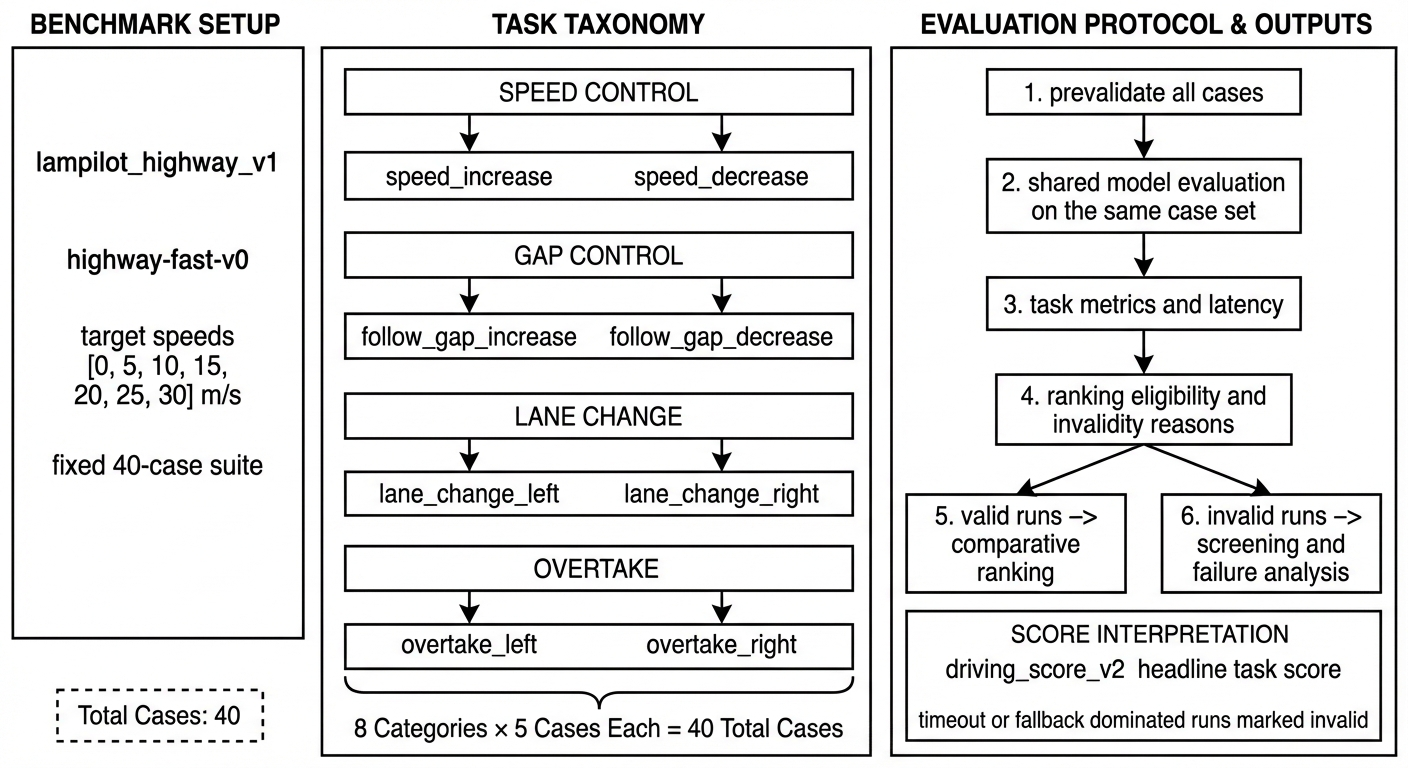
\includegraphics[width=\linewidth]{benchmark_test_specification.png}
\caption{Benchmark-test specification for the highway study. The figure summarizes the fixed \texttt{lampilot\_highway\_v1} suite, its task taxonomy, and the validity-aware evaluation path used for all model tiers. It is a benchmark-design figure rather than a performance summary.}
\label{fig:benchmark-test-specification}
\end{figure}

Within the valid subset, our headline task metric is \metric{driving\_score\_v2}, reported alongside task completion, crash rate, and mean decision latency. We do not collapse these into a single global score, and we do not rank invalid runs by latency alone. Instead, the design is deliberately layered. First, we ask whether a tier produces enough valid rows to support ranking at all. Second, for tiers that do, we use valid-only leaderboard-style comparisons to characterize the operating region that the benchmark can still compare fairly. Third, we ask whether any exact base-versus-fine-tuned pairs survive that screen and therefore support a causal fine-tuning interpretation. This staged procedure makes the logic of the paper explicit: screening comes before ranking, and ranking comes before adaptation claims.

This is why Table~\ref{tab:lightweight-leaderboard} and Figure~\ref{fig:cross-tier-pareto} function as main-paper evidence, whereas the midclass and highclass summaries are interpreted as screening and failure-analysis results rather than as symmetric benchmark tables. The lightweight assets describe the only tier in which multiple valid local models can still be ranked and interpreted together. The midclass table records which families retain at least one valid representative while simultaneously documenting why exact family-level attribution remains blocked. The highclass summary has a different purpose again: it demonstrates that the current local runtime regime can exhaust the benchmark's interpretability before a family-level comparison ever begins.

The resulting design is asymmetric by construction. Lightweight is the only tier that supports both comparative ranking and an exact pairwise fine-tuning test, with the Phi pair providing the paper's direct adaptation evidence in Table~\ref{tab:lightweight-pair-delta}. Midclass still offers partial visibility into valid local behavior, but not enough matched coverage for clean pairwise attribution. Highclass serves a different scientific role: it shows where the current local runtime regime causes the benchmark to stop producing interpretable rows altogether. We now turn to that screening structure and the small set of comparisons it actually licenses.

\section{Results}

\subsection{Three-tier screening overview}

The primary result is a validity gradient, not a leaderboard. Table~\ref{tab:validity-summary} shows that 7 of 14 lightweight models remain ranking-eligible, compared with 3 of 6 midclass models and 0 of 4 highclass models. Figure~\ref{fig:cross-tier-validity} makes the same pattern visually explicit: as model tier increases, the benchmark stops behaving like a stable ranking instrument and starts behaving like a runtime stress test. Fine-tuning cannot be interpreted independently of this screening structure, because strong pairwise conclusions are only possible inside the region where runs remain valid. Under the current local runtime policy, that region is concentrated in lightweight.

\begin{table}[t]
\caption{Cross-tier validity summary. This table reports ranking eligibility, not task quality alone, and defines where the benchmark supports ranking, screening only, or failure analysis.}
\label{tab:validity-summary}
\centering
\small
\begin{tabularx}{\linewidth}{lrrrrrl}
\toprule
Tier & Total & Valid & Invalid & Invalid frac. & Exact pairs & Interpretation \\
\midrule
Lightweight & 14 & 7 & 7 & 0.50 & 1 & results-ready \\
Midclass & 6 & 3 & 3 & 0.50 & 0 & screening-only \\
Highclass & 4 & 0 & 4 & 1.00 & 0 & failure-analysis-only \\
\bottomrule
\end{tabularx}
\end{table}

\begin{figure}[t]
\centering
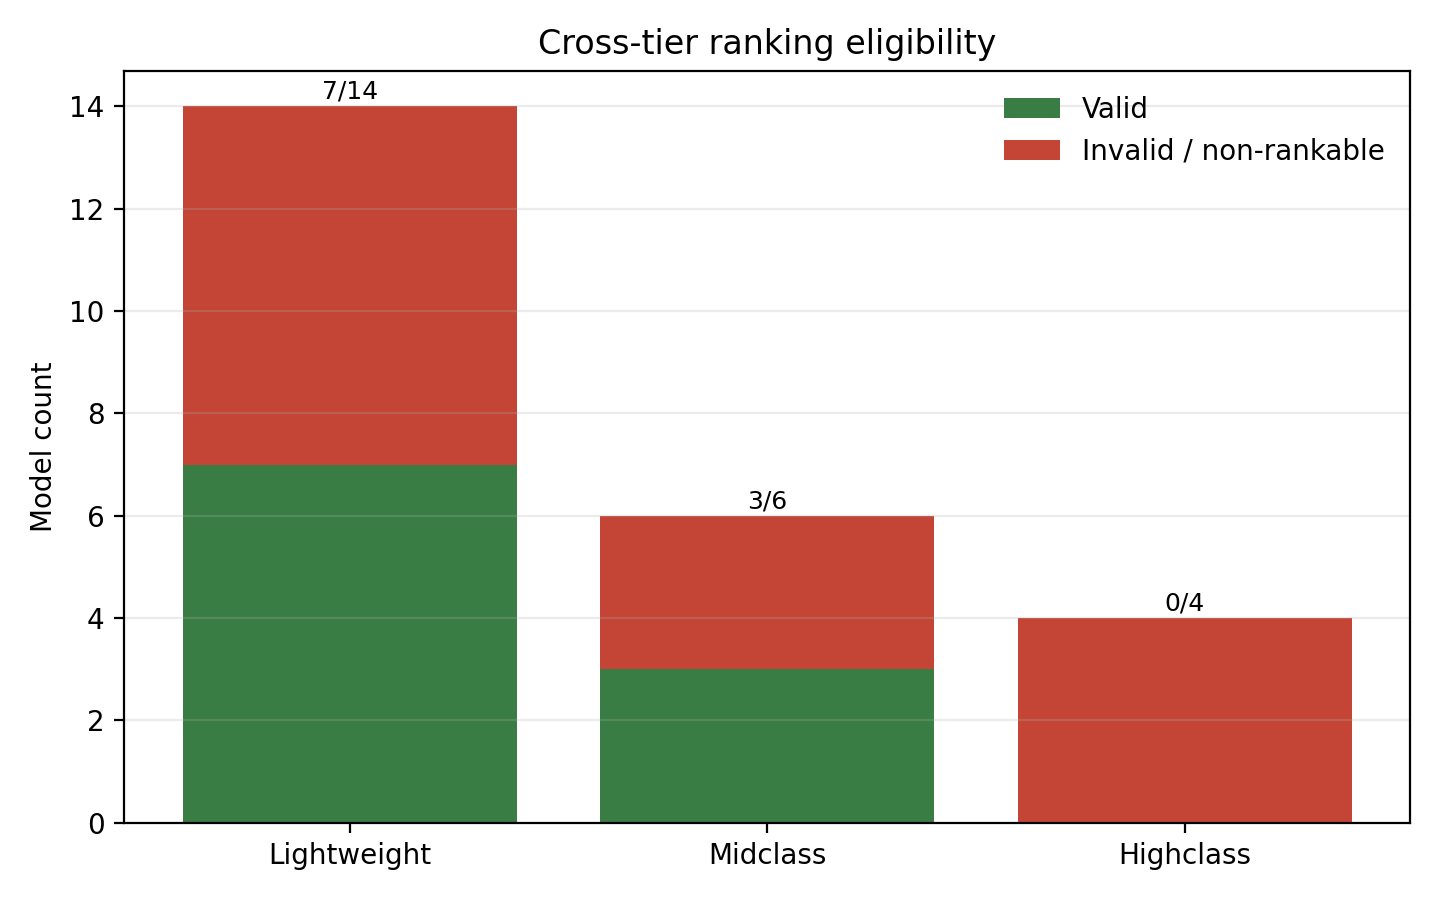
\includegraphics[width=0.92\linewidth]{cross_tier_validity.png}
\caption{Cross-tier validity summary. The figure visualizes ranking eligibility rather than task quality alone; the central pattern is collapse of valid comparison at larger scale under the current local runtime policy.}
\label{fig:cross-tier-validity}
\end{figure}

\subsection{Lightweight comparative evidence}

Lightweight is the only tier where the benchmark supports both comparative ranking and exact pairwise interpretation. Table~\ref{tab:lightweight-leaderboard} shows that Llama 3.2 3B Base is the top valid lightweight model in the current bundle, reaching \metric{driving\_score\_v2}~=~0.1403 with a task completion rate of 0.35 at roughly 1196 ms mean decision latency. Several fine-tuned lightweight models also remain competitive, notably DiLu Qwen3 1.7B v1 and DiLu Phi-4 Mini 3.8B Instruct v1. For coverage transparency, the same table also lists invalid lightweight rows beneath the ranked block with metric cells left empty; those rows document benchmark reach, but only valid rows contribute to ranking and the Pareto view. Figure~\ref{fig:cross-tier-pareto} shows why this tier matters: the lightweight story is not only about peak score, but about occupying the only part of the latency-quality frontier where multiple local models remain both valid and interpretable. In practice, lightweight is the only tier where the benchmark still behaves like the comparative instrument the fine-tuning question requires.

\begin{table*}[t]
\caption{Lightweight model inventory ordered by valid-row rank. Ranking-eligible models appear first and define the comparative leaderboard; invalid rows are shown below for coverage transparency with non-identity value fields left empty.}
\label{tab:lightweight-leaderboard}
\centering
\small
\resizebox{\textwidth}{!}{%
\begin{tabular}{r l l l r r r r}
\toprule
Rank & Model & Variant & Status & \metric{driving\_score\_v2} & Completion & Crash & Latency (ms) \\
\midrule
1 & Llama 3.2 3B Base & base & valid & 0.1403 & 0.350 & 0.350 & 1196.2 \\
2 & DiLu Qwen3 1.7B v1 & fine-tuned & valid & 0.1305 & 0.275 & 0.425 & 1502.8 \\
3 & DiLu Phi-4 Mini 3.8B Instruct v1 & fine-tuned & valid & 0.1257 & 0.350 & 0.575 & 1215.9 \\
4 & Llama 3.2 1B Base & base & valid & 0.0885 & 0.175 & 0.125 & 917.0 \\
5 & Phi-4 Mini 3.8B & base & valid & 0.0838 & 0.425 & 0.750 & 1322.2 \\
6 & DiLu DeepSeek R1 1.5B v3 & fine-tuned & valid & 0.0724 & 0.200 & 0.125 & 1519.6 \\
7 & DiLu Qwen3 4B v1 & fine-tuned & valid & 0.0706 & 0.175 & 0.825 & 1019.6 \\
\midrule
\multicolumn{8}{l}{\textit{Invalid lightweight rows shown for coverage only; these rows do not contribute to ranking.}} \\
\midrule
 & DeepSeek R1 1.5B Base & base & quarantined+incomplete+invalid &  &  &  &  \\
 & DiLu Llama 3.2 1B Instruct v1 & fine-tuned & quarantined+incomplete+invalid &  &  &  &  \\
 & DiLu Llama 3.2 3B Instruct v1 & fine-tuned & quarantined+incomplete+invalid &  &  &  &  \\
 & Phi-4 Mini Reasoning 3.8B & base & quarantined+incomplete+invalid &  &  &  &  \\
 & DiLu Phi-4 Mini 3.8B Reasoning v1 & fine-tuned & quarantined+incomplete+invalid &  &  &  &  \\
 & Qwen3 1.7B Base & base & quarantined+incomplete+invalid &  &  &  &  \\
 & Qwen3 4B Base & base & quarantined+incomplete+invalid &  &  &  &  \\
\bottomrule
\end{tabular}
}
\end{table*}

\begin{figure}[t]
\centering
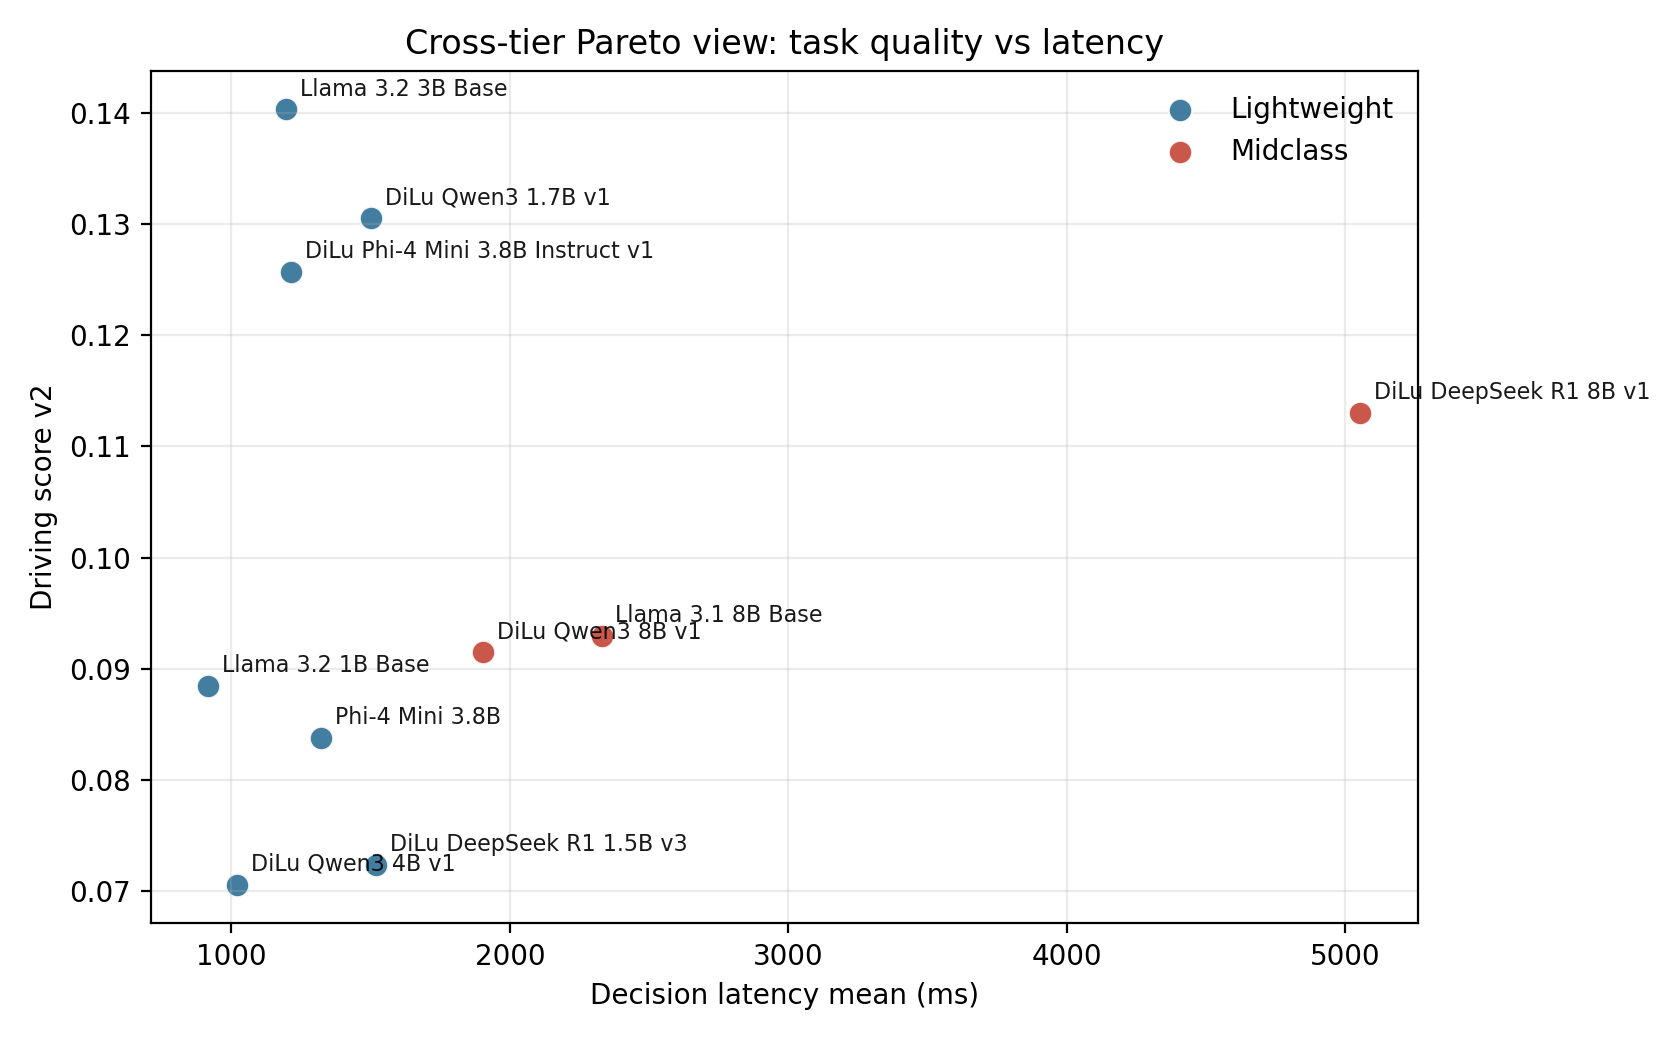
\includegraphics[width=0.92\linewidth]{cross_tier_pareto.png}
\caption{Cross-tier Pareto view of task quality versus latency using ranking-eligible models only. Highclass contributes no valid frontier points under the current local runtime regime.}
\label{fig:cross-tier-pareto}
\end{figure}

\subsection{Exact fine-tuning evidence in lightweight}

The Phi family provides the only exact eligible fine-tuning comparison in the current paper. Table~\ref{tab:lightweight-pair-delta} now lists all attempted lightweight base-versus-fine-tuned pairs, making the blocked comparisons explicit rather than leaving them implicit. Only the Phi-4 Mini 3.8B pair retains measurable deltas: DiLu Phi-4 Mini 3.8B Instruct v1 improves \metric{driving\_score\_v2} by 0.0419 and \metric{overall\_score\_mean} by 0.1006 relative to the base model, while also reducing mean decision latency by about 106 ms. This matters because it clears the paper's strictest evidential bar: both sides of the comparison are ranking-eligible under the same local runtime regime. That makes the Phi pair more than an anecdote. It is direct evidence that fine-tuning can improve a local driving agent without paying an obvious latency penalty. At the same time, the empty delta rows define the limit of the claim. The paper can argue for a real lightweight fine-tuning effect, but it cannot generalize that effect across families that never become jointly rankable.

\begin{table*}[t]
\caption{Lightweight base-versus-fine-tuned pair inventory. All attempted lightweight pairs are shown; delta fields remain empty when the pair is not jointly ranking-eligible. Positive values favor the fine-tuned model except for latency, where negative is better.}
\label{tab:lightweight-pair-delta}
\centering
\small
\resizebox{\textwidth}{!}{%
\begin{tabular}{l l l l l r r r r}
\toprule
Family & Base model & Fine-tuned model & Eligible & Pair issue & $\Delta$ \metric{driving\_score\_v2} & $\Delta$ completion & $\Delta$ overall & $\Delta$ latency (ms) \\
\midrule
DeepSeek & DeepSeek R1 1.5B Base & DiLu DeepSeek R1 1.5B v3 & no & base\_or\_fine\_tuned\_not\_rankable &  &  &  &  \\
Llama & Llama 3.2 1B Base & DiLu Llama 3.2 1B Instruct v1 & no & base\_or\_fine\_tuned\_not\_rankable &  &  &  &  \\
Llama & Llama 3.2 3B Base & DiLu Llama 3.2 3B Instruct v1 & no & base\_or\_fine\_tuned\_not\_rankable &  &  &  &  \\
Phi & Phi-4 Mini 3.8B & DiLu Phi-4 Mini 3.8B Instruct v1 & yes &  & +0.0419 & -0.0750 & +0.1006 & -106.3 \\
Phi & Phi-4 Mini Reasoning 3.8B & DiLu Phi-4 Mini 3.8B Reasoning v1 & no & base\_or\_fine\_tuned\_not\_rankable &  &  &  &  \\
Qwen & Qwen3 1.7B Base & DiLu Qwen3 1.7B v1 & no & base\_or\_fine\_tuned\_not\_rankable &  &  &  &  \\
Qwen & Qwen3 4B Base & DiLu Qwen3 4B v1 & no & base\_or\_fine\_tuned\_not\_rankable &  &  &  &  \\
\bottomrule
\end{tabular}
}
\end{table*}

\subsection{Midclass screening results}

Midclass is useful, but only as screening evidence. The best valid midclass model is DiLu DeepSeek R1 8B v1 with \metric{driving\_score\_v2}~=~0.1130, and Table~\ref{tab:midclass-screening} shows the full six-model inventory rather than only family-best survivors. Invalid rows are retained with blank value cells so that the missing exact eligible pairs remain explicit at the row level rather than being hidden inside aggregate summaries. The right interpretation is therefore not that midclass is uninformative, but that it reveals partial viability without clean causal comparison. Some 8B models can survive the benchmark and produce meaningful scores, yet the tier as a whole remains too brittle for the paper to claim a family-level fine-tuning effect. The benchmark is actively showing where interpretation stops being secure.

\subsection{Highclass failure analysis}

Highclass is not a failed leaderboard; it is a failure-analysis regime. None of the four tested 14B models are ranking-eligible in the current bundle, and Table~\ref{tab:highclass-failure} keeps all four rows visible with only identity and status text preserved. Leaving the other value fields empty makes the interpretation boundary explicit: these runs belong in a validity inventory, not in a comparative score table. Figure~\ref{fig:cross-tier-pareto} reflects the consequence directly: highclass contributes no valid points to the main frontier. This is not absent evidence. It is an empirical result about the scale boundary beyond which comparative claims about fine-tuning or model quality are no longer trustworthy under the current local runtime regime. That failure mode strengthens the paper's main argument by showing that runtime validity is part of what determines whether the benchmark is measuring policy quality at all.

\section{Discussion and Limitations}

The main methodological implication of this paper is that benchmark validity should be treated as part of intelligent-vehicle evaluation whenever the driving policy depends on local LLM inference. In a conventional simulation study, ranking is often assumed to be the natural endpoint of the experiment. Our results suggest a stricter interpretation for local language-model agents: before comparing policies, the evaluation must first establish that the runtime regime leaves those policies jointly interpretable. This does not replace scenario coverage, safety validation, or broader vehicle-level testing. It adds an additional layer of measurement discipline for language-driven controllers whose inference behavior can dominate the usefulness of the benchmark itself.

That implication also changes how fine-tuning results should be read in automated-driving research. A fine-tuned policy that improves score but does so only in the region where the evaluation remains stable is scientifically useful; a fine-tuned policy that cannot remain rankable under the intended local runtime regime is harder to justify as an evaluation win. The paper therefore argues for a narrower but more defensible reading of local adaptation: fine-tuning evidence should be attached not only to task improvement, but also to the validity conditions under which that improvement was observed.

The main limitation of the current paper is sparse exact pair coverage. Although the repository supports many model families and multiple tiers, only one exact base-vs-fine-tuned pair is ranking-eligible in the current evidence bundle. This means the fine-tuning story is real but still narrow. The paper should be explicit that family-level generalization remains unresolved.

The second limitation is scope. The repository contains cross-scenario infrastructure for merge and intersection tasks, but those settings are not part of the empirical evidence in the present manuscript. The first paper should therefore remain highway-only and avoid implying any cross-scenario generalization. For intelligent-vehicle evaluation, this also means the current study should be read as a targeted examination of local decision-making behavior in one highway benchmark family rather than as a complete validation protocol for automated driving.

A third limitation is runtime-regime specificity. The current timeout ladder, hardware context, and local serving stack are part of the studied setup. That is a strength for local reproducibility, but it also means the present manuscript should not present the resulting validity boundary as a universal benchmark standard. The paper can claim that runtime validity is a first-class measurement concern for local LLM driving agents; it cannot claim that the exact scale boundary observed here will transfer unchanged to every inference stack or vehicle-evaluation workflow.

\section{Conclusion}

DiLu-Ollama makes local-first evaluation of LLM driving agents more scientifically usable by combining simulation, task-conditioned benchmarking, runtime-aware validity handling, and publication-facing analysis. For intelligent-vehicle research, the central message is not only that local language-model policies can be benchmarked, but that the benchmark must also reveal when runtime behavior breaks the comparison itself. In the resulting three-tier highway study, lightweight is the only evidence-ready tier, midclass remains screening-only, and highclass exposes a runtime-scalability boundary rather than a competitive ranking. Within that evidence base, the Phi lightweight pair provides a concrete example that fine-tuning can improve local driving performance without increasing mean latency. The claim is intentionally narrow, but that is the point: fine-tuning gains are only meaningful inside the part of the model space where benchmark validity survives the local runtime regime.


\appendices
\section{Additional Screening Tables}

\begin{table*}[h]
\caption{Midclass model inventory. Valid rows retain their measured values, while invalid rows are shown with blank value fields so the missing exact eligible pairs remain explicit.}
\label{tab:midclass-screening}
\centering
\small
\resizebox{\textwidth}{!}{%
\begin{tabular}{l l l l r r}
\toprule
Family & Model & Kind & Status & \metric{driving\_score\_v2} & Latency (ms) \\
\midrule
DeepSeek & DeepSeek R1 8B Base & base & quarantined+incomplete+invalid &  &  \\
DeepSeek & DiLu DeepSeek R1 8B v1 & fine-tuned & valid & 0.1130 & 5054.2 \\
Llama & Llama 3.1 8B Base & base & valid & 0.0930 & 2329.5 \\
Llama & DiLu Llama 3.1 8B v1 & fine-tuned & quarantined+incomplete+invalid &  &  \\
Qwen & Qwen3 8B Base & base & quarantined+incomplete+invalid &  &  \\
Qwen & DiLu Qwen3 8B v1 & fine-tuned & valid & 0.0915 & 1903.5 \\
\bottomrule
\end{tabular}
}
\end{table*}

\begin{table*}[h]
\caption{Highclass model inventory. All 14B models are invalid under the current runtime regime, so only identity and status text are retained while value fields remain empty.}
\label{tab:highclass-failure}
\centering
\small
\resizebox{\textwidth}{!}{%
\begin{tabular}{l l l r r r r}
\toprule
Model & Variant & Status & \metric{driving\_score\_v2} & Completion & Crash & Mean latency (ms) \\
\midrule
DeepSeek R1 14B Base & base & quarantined+incomplete+invalid &  &  &  &  \\
DiLu DeepSeek R1 14B v1 & fine-tuned & quarantined+incomplete+invalid &  &  &  &  \\
DiLu Qwen3 14B v1 & fine-tuned & quarantined+incomplete+invalid &  &  &  &  \\
Qwen3 14B Base & base & quarantined+incomplete+invalid &  &  &  &  \\
\bottomrule
\end{tabular}
}
\end{table*}


\bibliographystyle{IEEEtran}
\bibliography{references}

\begin{IEEEbiographynophoto}{Anjie Qiu}
Anjie Qiu is pursuing the Ph.D. degree with RPTU Kaiserslautern-Landau, Kaiserslautern, Germany, where he has worked since 2019 on vehicular communication and artificial intelligence topics. He is also a Senior AI Architect working on mobility- and IoT-oriented research projects spanning prototype implementation, evaluation pipelines, benchmarking, and partner-driven demonstrators. He previously completed an internship with Daimler AG, Stuttgart, Germany, on data-engineering workflows for electric-powertrain diagnostics. His research interests include large language model evaluation, autonomous-driving simulation, connected mobility, vehicular communications, and reliable local AI systems for intelligent vehicles.
\end{IEEEbiographynophoto}


\end{document}
